\documentclass[12pt,spanish]{article}
\usepackage[spanish,activeacute]{babel}
\usepackage[utf8]{inputenc}
\usepackage{graphicx}

\title{\textbf{Técnicas de IA aplicadas a la robótica\\}Módulo de navegación}
\author{Pablo Francisco Pérez Hidalgo}
\date{20/03/2010}

\begin{document}
\maketitle
\begin{center}
	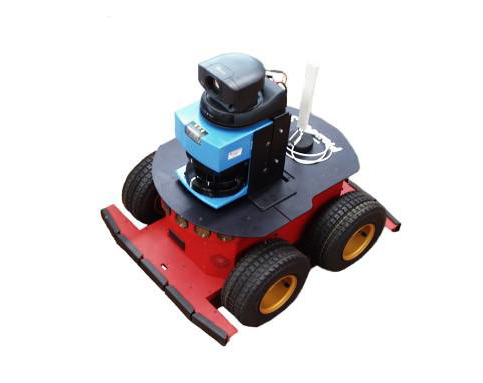
\includegraphics[scale=1.6]{./imagenes/pioneer.eps}
\end{center}
\newpage
\tableofcontents
\newpage
\section{Introducción}
No se van a comentar en este documento los objetivos del sistema de navegación ni su papel en el sistema global de controlador de un robot móvil. Estos aspectos forman parte del enunciado del problema y, por tanto, están descritos en dichos documentos.
Por ello, en esta sección de introducción, se tratará de realizar un mapa esquemático de la solución alcanzada en el desarrollo de este módulo.\\
\subsection{Objetivos y capacidades del módulo de navegación}
Lo primero es aclarar que el propósito del módulo de navegación desarrollado no vas más allá que el de hacer que el robot se acerque a un punto objetivo evitando chocar obstáculos, es por ello por lo que en la funcionalidad implementada no se encuentran ninguno de los siguientes aspectos:
\begin{itemize}
	\item Alcanzar el punto objetivo en circunstancias en las que se den mínimos locales, en lo que a la función objetivo del sistema reactivo de control respecta (dicha función objetivo es la distancia del robot al punto objetivo), esto es: No forma parte del navegador desarrollado el salir de situaciones en las que el robot tenga que posicionarse en puntos con distancias mayores del punto objetivo que distancias ya alcanzadas. Un ejemplo de esta situación puede observarse en la \textit{figura 1}.
	\begin{figure}[ht]
	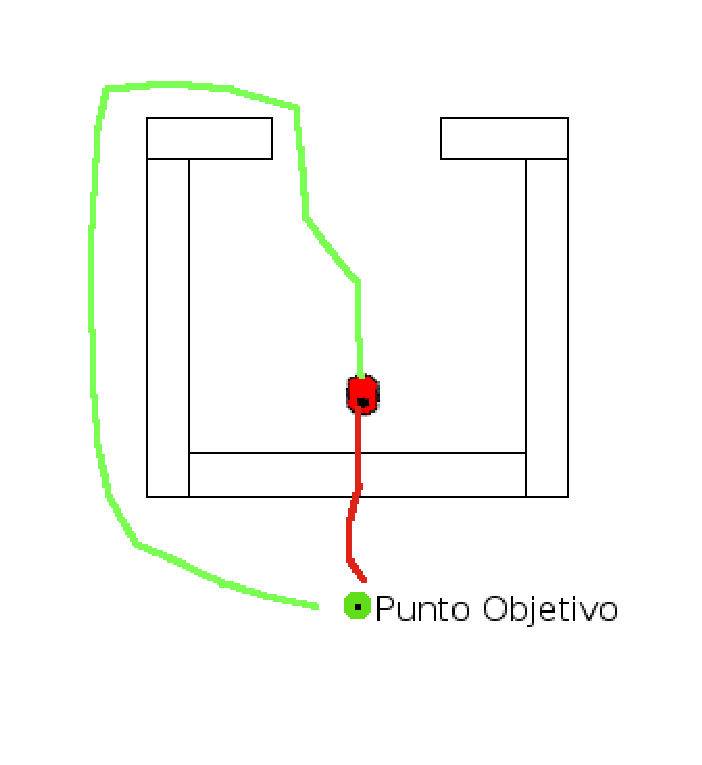
\includegraphics[scale=0.7]{./imagenes/minimoLocal.eps}
	\caption{La ruta en color verde indica el camino que el robot debería seguir para resolver la problemática del mínimo local (no implementado). El camino en color rojo representa lo que la implementación presentada del módulo de navegación plantea como solución al problema, como dicha implementación no va a permitir que el robot choque, no realizará ese camino y por lo tanto no resolverá la problemática.}
	\end{figure}
	\item Realizar planes para alcanzar objetivos no inmediatos o muy lejanos.
\end{itemize}
\subsection{Fundamentos de IA aplicados en sistema de navegación}
El sistema de navegación basa sus decisiones en los siguientes datos de entrada (inputs):
\begin{itemize}
	\item Posición del robot en el plano inferida a partir de:
	\begin{itemize}
		\item Posición inicial del robot al iniciar su "viaje".
		\item Datos de odometría.
	\end{itemize}
	\item Distancias a obstáculos medidas por medio de 8 sensores de ultrasonido.
	\item Diferencia angular entre el vector director del robot y el vector con origen en la posición del robot y con final en el punto objetivo.
\end{itemize}
Las salidas, o resultados de decisión, (outputs) afectan a dos actuadores que no son más que dos motores independientes manejados por medio de una abstracción software que permite indicar una velocidad de avance en línea recta y una velocidad de cambio de ángulo, en resumen, las salidas son:
\begin{itemize}
	\item Velocidad de giro $\in [-1.0,1.0] $
	\item Velocidad de avance $\in [-1.0, 1.0] $
\end{itemize}
Una vez modeladas las entradas y las posibles salidas que debe proporcionar el sistema, se puede proceder a detallar cómo se ha implementado la toma de decisión (salidas) dependiente de las entradas.
La solución escogida ha sido una red neuronal de tipo perceptrón con las siguientes características:
\begin{itemize}
	\item{\textbf{Capas: }} Capa de entrada (una neurona por entrada) y capa de salida (una única neurona correspondiente a la única salida).
	\item{\textbf{Entradas:} } 9 entradas en total, las cuales son:
		\begin{itemize}
			\item Lectura \textit{sónar} 0.
			\item Lectura \textit{sónar} 1.
			\item Lectura \textit{sónar} 2.
			\item Lectura \textit{sónar} 3.
			\item Lectura \textit{sónar} 4.
			\item Lectura \textit{sónar} 5.
			\item Lectura \textit{sónar} 6.
			\item Lectura \textit{sónar} 7.
			\item $\Theta = \hat{\vec{x},\vec{y}}$ con: $$ \vec{x} = \vec{VectorDirector}(Robot) ~~ \vec{y} = \vec{PosicionObjetivo}-\vec{PosicionRobot}$$
		\end{itemize}
	\item{\textbf{Salidas: }} Una única salida que representa la velocidad de giro ($V.Giro \in [-1.0, +1.0]$) dónde -1 ordena al robot que gire a la izquierda lo más rápido posible y +1 ordena al robot que gire a la derecha a máxima velocidad posible siendo los valores del intervalo $(0,1)$ giros a diversas velocidades hacia la derecha y los de $(-1,0)$ giros a diversas velocidades hacia la izquierda.
	\item{\textbf{Función de excitación de neurona de salida:} } $\sum_{i = 0}^{8}w_{i}\cdot x_{i}+b$ siendo $x_{i}$ la i-ésima entrada de la red.
	\item{\textbf{Función de activación:} } $tanh(excitacion)$ (ver \textit{figura 2}).
	\begin{figure}[!ht]
		\begin{center}
		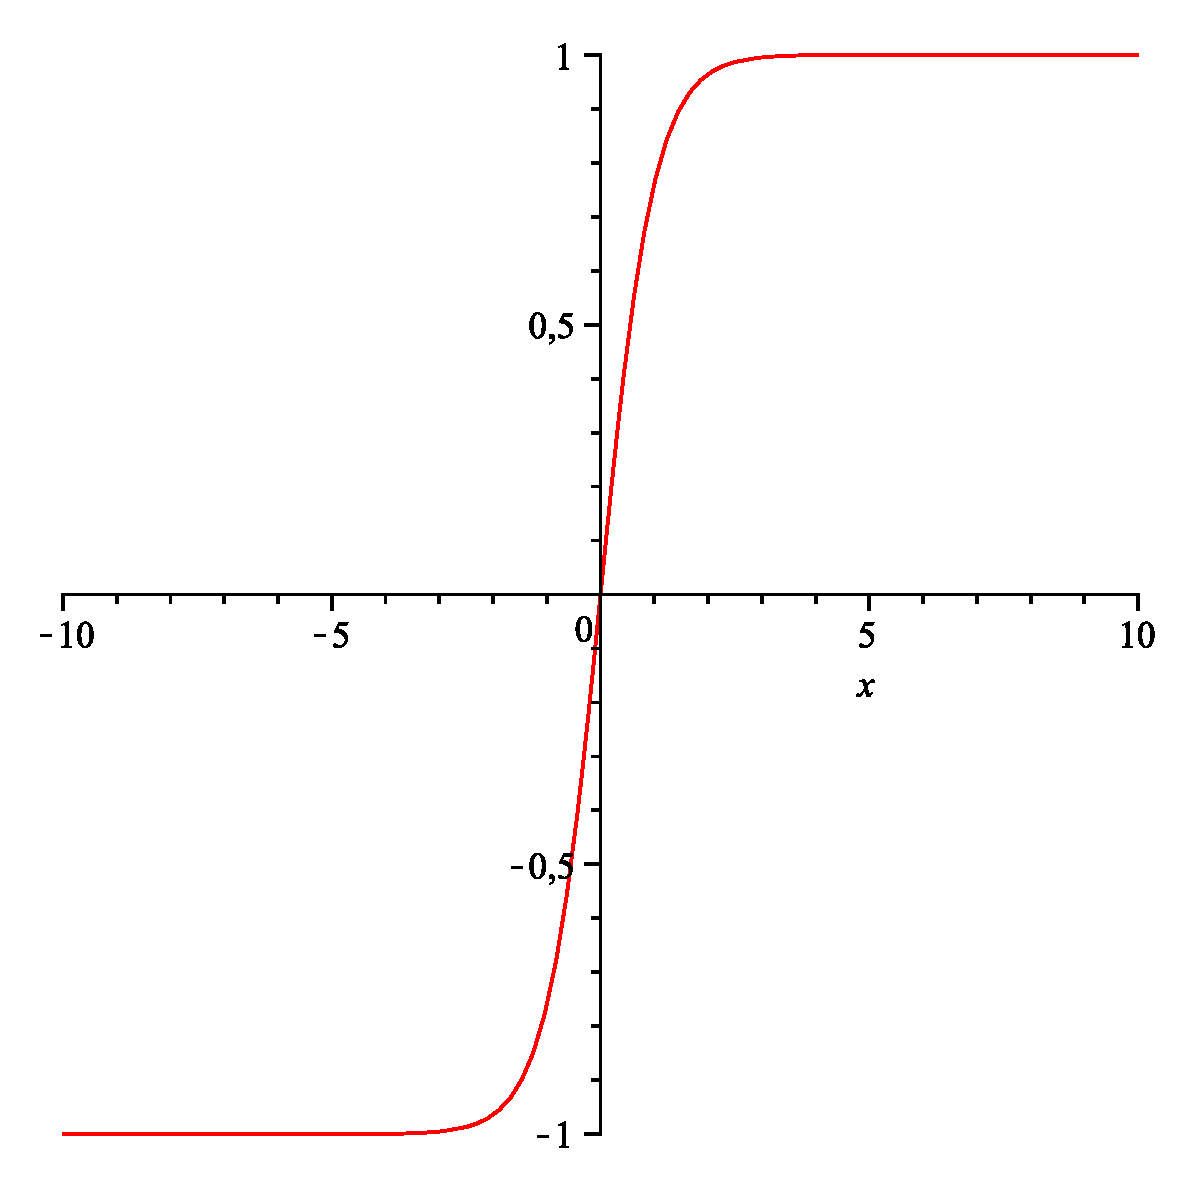
\includegraphics[scale=0.4]{./imagenes/activacion.eps}
		\caption{Representación de la función de activación utilizada.}
		\end{center}
	\end{figure}
	\item{\textbf{Representación esquemática del perceptrón: }}
	\begin{figure}[!ht]
		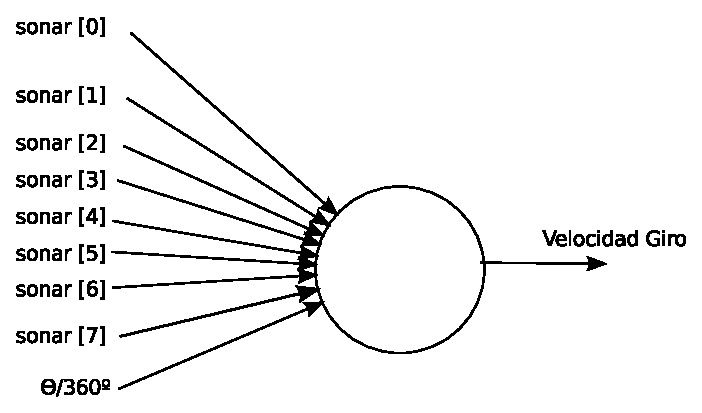
\includegraphics[scale=1.0]{./imagenes/perceptron.eps}
		\caption{Representación gráfica de la red neuronal}
	\end{figure}
\end{itemize}
\newpage
Del esquema de la \textit{figura 3} se desprende que la red neuronal sólo sirve para tomar decisiones sobre la velocidad de giro del robot, no obstante, el sistema de control debe ser capaz de determinar una velocidad de avance. Para ello, en ninguna de las soluciones presentadas en este documento se ha utilizado una red neuronal, se han usado dos funciones de velocidad de avance totalmente algorítmicas y computables:
\begin{itemize}
	\item Una primera solución, la más trivial, es que la velocidad de avance sea constante en tanto que no se haya alcanzado el punto objetivo y que sea nula ($Vel.Avance = 0 m/s $) cuando el robot se encuentra en un entorno muy cercano al punto objetivo, considerando así que el objetivo ha sido alcanzado. Así pues, la velocidad de avance vendrá dada por la siguiente función:
	$$V.Avance = \left\{ \begin{array}{ll}
							0.5 & \textrm{Si } distancia(robot,objetivo) > \varepsilon \\
							0 & \textrm{Si } distancia(robot, objetivo) \le \varepsilon \\
						   \end{array} \right.$$
	Con $\varepsilon \to 0$.
	\item La solución anterior presenta algunos problemas que se comentarán en secciones posteriores, por ello se plantea otra posible solución en la cual, la velocidad de avance depende de la velocidad de giro:
	$$
	V.Avance = \left\{
				\begin{array}{ll}
				f(V.Giro) & \textrm{Si } distancia(robot,objetivo) > \varepsilon\\				
				0 & \textrm{Si } distancia(robot,objetivo) \le \varepsilon\\
				\end{array}
				\right.
	$$	
	Con $\forall x \in R, f(x) \in [-1,1]$ y $\varepsilon \to 0$.
\end{itemize}
Una vez planteada la estructura del sistema de toma de decisiones, lo más importante es conocer la configuración adecuada de este para que cumpla nuestros objetivos de alcanzar un punto destino evitando, en la manera de lo posible, los obstáculos que encuentre a sus paso.
En un sistema cuyas decisiones son tomadas gracias a una red neuronal, sea del tipo que sea, una configuración no es más que un vector de pesos, el vector de todos los pesos que ponderan las diversas entradas de las neuronas para dar lugar a la excitación de estas. La forma de obtener estos pesos constituirá el contenido fundamental del resto de este documento.
\section{Obtención de configuración para el perceptrón:\\Aprendizaje de la red neuronal}
En todo el desarrollo del módulo de navegación, la filosofía aplicada para el aprendizaje de la red neuronal ha sido la de la utilización de algoritmos genéticos. No se ha utilizado el algoritmo de aprendizaje supervisado clásico del perceptrón. El haberlo utilizado hubiera requerido un vector de respuestas por cada posible situación representativa en las entradas. Debido a que el robot recibe información de 8 sensores más un ángulo objetivo, esto hubiera dado lugar a una explosión combinatoria teniendo un vector de respuestas representativas extremadamente extenso.\\
No es objetivo de este documento el describir en qué consisten los algoritmos genéticos o evolutivos, lo que si se muestra en el siguiente listado es el conjunto de características que determinan el tipo de algoritmo genético utilizado:\\
\begin{itemize}
	\item{\textbf{Fenotipos o individuos:} Los individuos de la población serán los diversos percetrones para toma de decisión.}
	\item{\textbf{Genotipo:} El genotipo de cada perceptrón (individuo) es el vector de pesos neuronales que lo describe.}
	\item{\textbf{Evolución del tamaño de la población: }} Se considerará una población de tamaño constante.
	\item{\textbf{Operadores aplicados sobre la población:} }
		\begin{itemize}
			\item{\underline{Mutación: }} Un porcentaje (configurable) de la población muta parte de sus genes según una distribución normal. Si se utiliza elitismo, la élite siempre es subconjunto de la población no mutante.
			\item{\underline{Reemplazo: }} Todo individuo que muta es reemplazado por el mutante que da lugar. Si se utiliza elitismo, los miembros del subconjunto élite nunca serán remplazados puesto que nunca mutan. 
		\end{itemize}
	\item{\textbf{Condición de parada:} } El algoritmo parará cuando haya transcurrido un número configurable de generaciones habiendo o no encontrado una solución válida, es decir, un individuo adaptado al medio.
\end{itemize}  
En las ulteriores subsecciones se indican las diveras aplicaciones del algoritmo genético: los parámetros aplicados, la gestión de velocidad de avance, etc. 
\subsection{Primera aproximación}
Debido a que los primeros intentos suelen ser los más simples, la primera configuración utilizada del algoritmo genético carecía de elitismo, es decir, todos los individuos estaban sujetos a mutación y, salvo que la generación de números aleatorios según la distribución normal diese lugar a un vector compuesto únicamente de ceros (suceso con probabilidad teórica 0 ya que la probabilidad de un valor en una distribución continua es 0), no había ni un sólo individuo que no fuese modificado en mayor o menor medida de una generación a otra. Esto da lugar al continuo descarte de soluciones aunque estas sean válidas, los individuos mejor adaptados no tenían ventajas sobre los peores lo cual no genera ningún tipo de evolución. Esta primera aproximación, totalmente errónea y aparentemente infructuosa, sirvió para establecer y desarrollar los mecanismos software que permiten utilizar el algoritmo general pero en diferentes versiones con tan solo modificar algunos parámetros en la función de inicialización del "cerebro" o, como se llama en \textit{pyro}, "brain".\\
Además de las observaciones, esta primera aproximación tenía las siguientes características:\\
\begin{itemize}
	\item{\textbf{Histórico de individuos que alcanzaron alguna vez el punto objetivo:} } En un principio, esta característica se añadió por motivos de depuración, pero en tanto que la primera aproximación iba siendo depurada se utilizó para determinar cual había sido el mejor individuo de entre todas las poblaciones de todas las generaciones. El histórico no es más que una colección de pesos (genotipos) con el valor de fitness que habían obtenido al alcanzar al menos un objetivo. Así pues, cada vez que un robot alcanzaba un punto objetivo sin haber chocado su genotipo (configuración del perceptrón) y el "fitness" obtenido eran anotados en dicha lista. Tras finalizar la última generación se tomaba a aquel individuo con mayor "fitness" de dicho histórico como mejor individuo.
	\item{\textbf{Función Fitness:} } La primera función de cálculo de "fitness" utilizada es la descrita por la siguiente expresión:
	$$fitness(individuo) = \left\{
		\begin{array}{ll}
			10^{-4}\cdot nºTicks(individuo) & \textrm{Si el individuo ha chocado} \\
			10^{-3}\cdot \frac{1}{nºTicks(individuo)} & \textrm{Si el individuo no ha chocado pero }\\
			 &  nºTicks(individuo) > limiteTicks\\
			\frac{distancia(posInicial,posDestino)}{nºTicks(individuo)} & \textrm{Si el individuo}\\
			 & \textrm{ha llegado a su destino}
		\end{array}
	\right.$$
	\item{\textbf{NºGeneraciones: }} Se ha probado con 20, 50, 200, 500 y 1000 (En el código fuente, este parámetro viene dado por la variable `g`).
	\item{\textbf{Tamaño de la población: }} Se ha probado con poblaciones de 10 individuos (En el código fuente, este parámetro viene dado por la variable `N`).
	\item{\textbf{Determinación de velocidad de avance: }} Aunque este apartado no tiene nada que ver con el algoritmo evolutivo, conviene incluirlo en esta lista como resumen de la solución planteada. En esta solución se utilizó la opción de velocidad de avance constante (0.5).
\end{itemize}
Conviene analizar el por qué de haber tomado la función de "fitness" presentada en la enumeración anterior. El robot puede intentar acometer su tarea de llegar al punto objetivo con tres resultados posibles:
\begin{enumerate}
	\item{\underline{El robot choca:} } En este caso, el valor de "fitness" debería ser 0 ya que no se desean individuos que no sean capaces de evitar obstáculos. No obstante, en un principio se pensó en incentivar de alguna forma (dándole un valor ínfimo "fitness" en vez de 0) a aquellos individuos que tardasen más en chocar ,por ello en el caso de choque la función de evaluación del individuo es directamente proporcional al número de ticks que este ha realizado, eso si, la constante de proporcionalidad es extremadamente baja ($10^{-4}$).
	\item{\underline{El robot no choca pero no alcanza a su objetivo en un número de ticks máximo:} }En este caso se pretende incentivar el hecho de que no choquen    por lo que los individuos no reciben una valoración nula. Por otro lado, se pretende dar ventaja a aquellos individuos que, sin chocar, han realizado menos recorrido, por ello, su valor de ajuste es inversamente proporcional al número de ticks que han realizado antes de morir por inanición. Dado que la inanición se controla por un número de ticks máximo, todos los individuos que entran en bucle obtienen la misma valoración de ajuste.
	\item{\underline{El robot llega a su objetivo:} } En este caso el robot debe obtener la puntuación más alta ponderada, sin embargo, por medio de la relación $\frac{distancia(posRobot,posObjetivo)}{NºTicks}$ que representa la velocidad del robot en realizar su recorrido, de forma que los individuos que realizan recorridos más óptimos que otros obtienen mayores puntuaciones.
\end{enumerate}
\begin{tabular}{|l|}
\hline
\textbf{NOTA:}\\
Es muy importante tener en cuenta, en esta solución y en todas las presentadas\\
en este documento, que cada vez que se calcula la función de ajuste de in individuo\\
al medio no siempre se realiza la misma ruta, sino que se ordena al individuo que\\
afronte una ruta u otra según una función pseudoaleatoria que selecciona una de las\\
4 tuplas origen-destino de la colección de pruebas. Esta colección de tuplas\\
origen-destino contiene los casos más representativos que pueden darse ante la\\
presencia de obstáculos.\\
\hline
\end{tabular}\\
\\
Tras probar con un número elevado de generaciones, se pudo deducir que el mejor individuo dado como el de mayor "fitness" de entre los presentes en el histórico de alcances ni siquiera era capaz de evitar los obstáculos, a lo sumo podía solventar situaciones concretas pero nada más. Esto, como ya se ha comentado, se debe al hecho de que no permanecen inmutables los individuos con mejor valor de ajuste de cada generación, lo cual se conoce como \textbf{elitismo}. Por ello, las siguientes dos soluciones (incluida la solución final) hacen uso de esta característica poblacional. El que no se use elitismo no quiere decir que no se converja hacia una solución pero si implica el que esta convergencia sea muy lenta, tanto que el algoritmo se aproxima a un algoritmo de exploración por fuerza bruta en el que no se aprovechan los avances de los individuos más aventajados sino que se prueba con muchos individuos diferentes hasta alcanzar uno (por azar) que cumple los requisitos del controlador.
\\
\\
\begin{tabular}{|l|}
\hline
\textbf{NOTA:}\\
La función $nºTicks(individuo)$ devuelve el número de "pasos"\\
(concepto de \textit{pyrobot}) que ha realizado el robot antes del\\
evento choque, muerte por demasiados pasos (inanición) ó llegada a\\
objetivo.\\
\hline
\end{tabular}
\subsection{Segunda aproximación: Elitismo}
Tras los malos resultados arrojados por la primera aproximación del algoritmo evolutivo de entrenamiento, se decide utilizar elitismo con el fin de que las generaciones nuevas aprovechen los avances realizados por sus antecesores. De esta forma, se añade un parámetro del algoritmo conocido como \textit{tasa de mutación}, este parámetro indica la proporción ($tasaMutantes \in (0,1)$) de la población que muta de una generación a otra, es decir, que no pertenece a la élite. Así pues, se define a la élite como al \textbf{subconjunto de la población que sobrevive a su generación, pasando a la siguiente, sin sufrir ningún tipo de cambio en su genotipo}.\\
En el siguiente listado se resumen las características de esta última especificación del algoritmo de entrenamiento evolutivo:\\
\begin{itemize}
	\item{\textbf{Función Fitness:} }\\
	$$fitness(individuo) = \left\{
		\begin{array}{ll}
			0.0 & \textrm{Si el individuo ha chocado}\\
			\frac{10}{nºTicks(individuo)} & \textrm{Si el individuo no ha chocado y}\\
			 & nºTicks(individuo)>limiteTicks\\
			fitness(individuo)_{UltimoCalculo} & \textrm{Si el individuo} \\
			 + 10\cdot \frac{distancia(posInicial,posDestino)}{nºTicks(individuo)} & \textrm{ha llegado}\\
			 & \textrm{a su destino}
		\end{array}
	\right.$$
	\item{\textbf{NºGeneraciones: }} El algoritmo converge hacia una solución aceptable, aproximadamente,sobre la generación 50.
	\item{\textbf{Tamaño de la población: }} Se ha probado con varios tamaños de población, aunque con un número de generaciones máximo igual a 50 y \textbf{35 individuos} se alcanza la solución.
	\item{\textbf{Determinación de velocidad de avance: }} Se utiliza la opción de velocidad de avance constante (0.5).
\end{itemize}
Al igual que en el caso anterior, la elección de la función "fitness" merece algunos comentarios. Esta vez, un individuo que choca obtiene la peor puntuación de adaptación posible (0). A su vez, los individuos que mueren por inanición son puntuados con un muy pequeño y constante con el fin de incentivar el hecho de que no choca con ningún obstáculo. La parte más novedosa y que, por tanto, merece más atención en estos comentarios es la puntuación de "fitness" 	que se le da a los individuos que no han chocado. En una de las anotaciones anteriores se comentaba que un individuo se probaba en una ruta (origen-destino) escogida mediante una función peseudoaleatoria, así pues, un individuo que haya pasado inmutable de una generación a otra puede cumplir que haya sido eficaz para las ruta que le fue asignada en la prueba de la generación anterior pero no para la ruta que le ha "tocado" seguir en la actual. Es por eso por lo que individuos que han obtenido una buena puntuación en una generación, pueden obtener un "fitness" 0 en la siguiente o siguientes. De todo ello se deducen las siguientes reglas para favorecer la evolución de la población hacia una solución adecuada al objetivo del sistema controlador:
\begin{itemize}
	\item Si un individuo choca, aunque en otra generación obtuviese una buena puntuación de ajuste, a este le es asignada la puntuación 0 en "fitness".
	\item Es bueno favorecer, frente a los demás, a aquellos fenotipos que hayan llegado al objetivo sin chocar en más de una ocasión.
\end{itemize}
La primera regla provoca que, ante choque, el individuo tenga puntuación "fitness" 0 y la segunda regla da lugar al aspecto más interesante de esta nueva función "fitness" y es que aquellos individuos que no chocan y alcanzan su objetivo acumulan puntuación de una generación a otra. Eso da lugar al primer término de la tercera rama de la función de ajuste al medio. En esta rama, $fitness(individuo)_{UltimoCalculo}$ indica el valor de "fitness" que el fenotipo obtuvo en la generación anterior.\\
Esta aplicación del modelo evolutivo ha conseguido dar buenos resultados en nuestra búsqueda de un controlador reactivo planteando una única limitación, esta limitación no tiene que ver con la forma de entrenar la red neuronal, ni siquiera tiene que ver con los aspectos controlados por la red neuronal (velocidad de giro) sino con el hecho de utilizar una velocidad de avance constante. Cuando se utiliza una velocidad de avance constante los movimientos de giro más extremos (es decir) con mayor relación entre variación de ángulo y avance del robot que se pueden conseguir son circunferencias con un radio directamente proporcional a la velocidad de avance. De esta forma se genera un dilema: Cuanto mayor es la velocidad de avance menor es la libertad de movimientos (giros restringidos a circunferencias de radio mayor) pero más lento es el proceso de alcance de objetivo. Este es el motivo de una tercera aproximación, o iteración del refinado del algoritmo.
\section{Tercera aproximación: Modificación dinámica de velocidad de avance}
Tal y como se comentó en la subsección anterior, una velocidad de avance constante provoca limitaciones en la libertad de movimientos. Con tal de solucionar estas limitaciones, en una clase presencial, el profesor  \textit{Nik Swoboda} sugirió que la velocidad de avance dependiese de la velocidad de giro, haciendo corresponder a una alta velocidad de giro una velocidad de avance baja y viceversa. De esta forma se pueden dar movimientos de rotación sin avance. La solución aplicada para el control dinámico de la velocidad de avance queda descrita según la siguiente expresión:\\
\begin{eqnarray}
	V.Giro = RedNeuronal(senrores,\Theta);\\
	V.Avance = 0.1+0.9*(1-|V.Giro|);
\end{eqnarray}
Realmente, con esta aplicación no se consiguen movimientos de rotación sin avance ya que siembre hay una pequeña componente constante en la velocidad de avance ($0.1$). Esto se ha hecho así para evitar, en el algoritmo evolutivo, individuos que lo único que hacen es girar sin avanzar ya que, aunque estos individuos son descartados en muertes por inanición, generan muchos retrasos que en la simulación en tiempo real (que es la técnica sobre la cual se ha utilizado el algoritmo evolutivo) provoca largas esperas.
En lo que respecta al resto de características, el algoritmo de la tercera aproximación es exactamente igual al de la segunda.
\section{Resultados finales}
Con la tercera aproximación comentada se obtiene una solución aceptable a partir de la generación 40 con una población de 35 individuos. El vector de pesos final viene dado en la siguiente tabla:\\
\\
\begin{tabular}{|c|c|c|c|c|c|c|c|c|c|}
\hline
\textbf{s[0]} & \textbf{s[1]} & \textbf{s[2]} & \textbf{s[3]} & \textbf{s[4]} & \textbf{s[5]} & \textbf{s[6]} & \textbf{s[7]} & \textbf{$\frac{\Theta}{360.0}$} & b\\
\hline
-0.258 &  1.1605 &  -0.1555 &  1.2578 &  -0.5570 &  -2.9552 &  -1.6809 &  -2.2014 &  -1.5535 &  1.2828\\
\hline
\end{tabular}
\end{document}